\documentclass[12pt]{article}
\usepackage{ctex}%引入中文字符的包
\usepackage{enumerate}%引用标号需要引入的包
\usepackage{amsmath}
%\usepackage{array}
\usepackage{graphicx}%用来在文档中插入图片
\usepackage{caption}%修改图注相关
\usepackage{subfigure}%用来插入并列的图片
\usepackage{float}%确定图片是否为浮动,而不是在一个固定的地方
\usepackage[a4paper,left=31.8mm,right=31.8mm,top=25.4mm,bottom=25.4mm]{geometry}
\begin{document} 
\begin{titlepage}
\begin{center}      
{\Huge \bfseries 机器学习实验报告}\\[1cm]
{\Large \bfseries 逻辑回归(Logistic Regression)}\\[10cm]
{\Large 姓名:秦海滨}\\[1cm]
{\Large 学号:1180300523}\\[8cm]
{\Large 2020年10月19号}
\end{center}
\end{titlepage}
\newpage
\tableofcontents
\newpage
\section{实验目的}
理解逻辑回归模型,掌握逻辑回归模型的参数估计算法。
\section{实验要求及环境}
\subsection{实验要求}
实现两种损失函数的参数估计(无惩罚项和有惩罚项的情况),可以采用梯度下降、共轭梯度或者牛顿法等。
\subsection{实验环境}
\noindent 操作系统:Windows10 \par
\noindent 开发环境:Spider 4.1.4,Python 3.8 \par
\section{基本思想}
逻辑回归(Logistic Regression)是一种解决分类问题的算法,虽然它的名字中带有“回归”二字,但实际上是利用回归的方法解决分类的问题。能通过不断的优化寻找最优的参数以正确地进行数据分类。常见的可以利用逻辑回归解决垃圾邮件分类问题(二分问题)、用户点击率(二分问题)问题。\par
实际上在之前的学习中我们就已经接触过一种回归问题,即“线性回归”。线性回归就是给定一系列数据,通过求取一个合适的线性函数,使其尽可能多地包含所有的数据,线性函数的表达式如下:
\[f(x)=w^Tx+b\]\par
其中,$w$和$b$都是通过学习得到的,我们常用的方法即是最小二乘法,通过最小化数据与模型的均方误差,求得优化后的参数。\par
实际上,“逻辑回归=线性回归+Sigmoid函数”。线性回归是一类回归问题,需要我们输出一条连续的曲线以表示数据中变量与变量间的关系;而逻辑回归是一类分类问题,通过数据中各特征维度的值对数据进行分类,输出的是对原始数据的划分结果。由于在线性回归模型中$f(x)=w^Tx+b$的值域是$\lbrack-\infty,+\infty\rbrack$,我们可以根据线性回归模型得到任意的一个值;但在逻辑回归中,我们需要通过概率对数据进行分类,即模型的值域应该在$\lbrack0,1\rbrack$内。此时我们引入Sigmoid函数,其表达式为:
\[sig(t)=\frac{1}{1+e^{-t}}\]\par
其函数图像如下:
\begin{figure}[H]
    \centering
    \subfigure[Sigmoid函数]{
    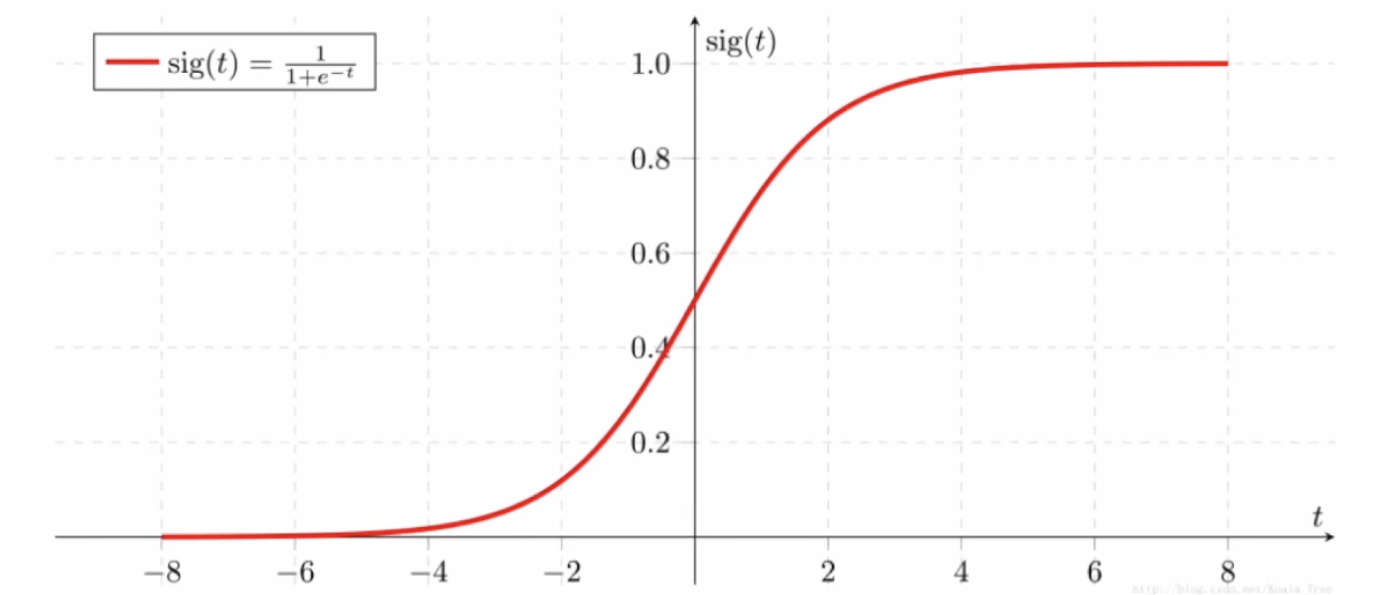
\includegraphics[width=0.8\textwidth]{Sigmoid.png} 
    }
\end{figure}
其连续性以及可导性在之后的优化中显得格外重要。\par
此时我们就可以将线性回归的回归问题转化为一个逻辑回归的分类问题:
\[sig(w^Tx+b)=\frac{1}{1+e^{-(w^Tx+b)}}\]\par
我们将Sigmoid函数的输出视作概率值作为分类的判断依据,若sig输出大于等于0.5,则将其视为正例;若sig输出小于0.5,则将其视作反例。\par
现在我们要做的,就是在给定样本集的基础上,通过学习、优化求出最优的参数$w^*$和$b^*$,使该模型能够对其他的样本输入做出分类。
\section{数据的生成}
可以通过输入不同类别的每一维数据的均值$\mu$和方差$\sigma$以单独生成满足高斯分布的数据。最后将多个类别的数据混合之后返回。\par
实验要求我们生成满足朴素贝叶斯假设的数据和不满足朴素贝叶斯假设的数据以测试逻辑回归的结果,我们可以通过调整输入的协方差矩阵以输出需要的数据类型。\par
\section{损失函数}
由于逻辑回归解决的是分类问题,所以其损失函数也是按照分类情况进行计算的。以二分类为例,我们定义逻辑回归的损失函数如下:\par
\[cost_i=\begin{cases}
    -ln(p_i),&if\ y_i=1\\
    -ln(1-p_i),&if\ y_i=0
\end{cases},\ p_i=\frac{1}{1+e^{-(w^Tx_i+b)}}\]\par
其中p表示Sigmoid函数的输出,即代入数据x算出的将其分为第一类($y_i=1$)的概率值。这个公式表示,若数据属于第一类($y_i=1$),则此时判断出的p越小,cost越大;若数据属于第0类(y=0),则此时判断出的p越大,cost越大。为了方便计算,我们将这个分段函数记为:
\[cost_i=-y_iln(p_i)-(1-y_i)ln(1-p_i)\]\par
所以对于一个给定的样本,我们可以计算样本集内所有数据的损失,即对所有的数据点的损失值求和,但在实际实验过程中我们会发现直接求和会导致溢出问题,故我们在公式前加上一定的系数防止溢出,如下:
\[COST=-\frac{1}{m}\sum_{i=1}^m(y_iln(p_i)+(1-y_i)ln(1-p_i))\]\par
我们也可以通过最大似然估计方式对参数进行估计,最终得出的公式与以上公式类似。\par
可以证明,以上得出的COST函数是关于w和b的凸函数,我们可以通过梯度下降法求出使COST函数取最小值时的参数$w^*$和$b^*$,构建出指定样本集上的逻辑回归模型。\par
为了方便计算,我们记常数项$b$为$w$中的第0维参数,即$w_0$,并在数据x中添加相应的维度,将$p_i$转换为如下形式:
\[p_i=\frac{1}{1+e^{-w^Tx_i}},\ 
w=\begin{bmatrix}
    w_0\\w_1\\\dots\\w_n
\end{bmatrix},\ 
x_i=\begin{bmatrix}
    1\\x_{i1}\\\dots\\x_{in}
\end{bmatrix}\]\par
这样,损失函数COST的取值便只与$w$的取值有关,我们可以记该函数为$COST(w)$,我们只需要求解出使损失函数最小的参数$w^*$即可。
\section{梯度下降法}
与Lab1中类似,在第i+1论的迭代中的梯度下降的公式如下,其中$\eta$为步长(即学习率):
\[w_{i+1}=w_i-\eta\frac{\partial\ COST(w)}{\partial w}\]
\subsection{不带惩罚项}
将Sigmoid公式代入到COST公式中化简,我们可以将COST的公式化简为如下向量形式:
\[COST(w)=-\frac{1}{m}\sum_{i=1}^{m}((1-y_i)w^Tx_i-ln(1+e^{w^Tx_i}))\]\par
对该式求导有:
\[\frac{\partial\ COST(w)}{\partial\ w}=-\frac{1}{m}\sum_{i=1}^mx_i((1-y_i)-\frac{e^{w^Tx_i}}{1+e^{w^Tx_i}})\]\par
将求出的导数代入到梯度下降的公式中,我们可以通过不断的迭代求出使$COST(w)$最小的$w^*$的值。为了防止无限的迭代,需要我们设置相应的最大迭代次数以及迭代精度。
\subsection{带惩罚项}
为了防止过拟合现象,我们需要为模型添加一定的惩罚项。类似于Lab1中添加惩罚项的方式,我们将损失函数修改为以下形式:
\[COST(w)=-\frac{1}{m}\sum_{i=1}^{m}((1-y_i)w^Tx_i-ln(1+e^{w^Tx_i}))+\frac{\lambda}{2m}w^Tw\]\par
求导的结果为:
\[\frac{\partial\ COST(w)}{\partial\ w}=-\frac{1}{m}\sum_{i=1}^mx_i((1-y_i)-\frac{e^{w^Tx_i}}{1+e^{w^Tx_i}})+\frac{\lambda w}{m}\]\par
与不带惩罚项的迭代方式相同,我们可以求解出$w*$的值,加入惩罚项后的模型在理论上应该有着防止过拟合的能力,我们会在后续的实验结果分析中对其进行验证。
\section{实验结果分析(以二分类为例)}
\subsection{实验数据满足朴素贝叶斯假设}
在生成数据之后,按照3:7的比例将数据集分割为训练集和测试集,共生成了1000个测试数据,数据均有两个特征。设置超参数为$\lambda=0.002$,测试结果如下:
\begin{figure}[H]
    \centering
    \subfigure[满足朴素贝叶斯假设的训练集测试结果]{
    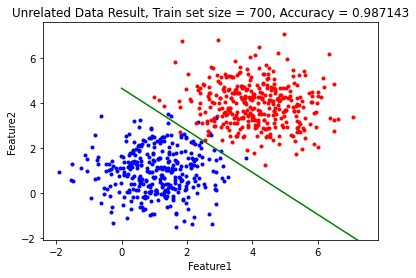
\includegraphics[width=0.6\textwidth]{Unrelated_Data_Result_Train.png}
    }
    \subfigure[满足朴素贝叶斯假设的测试集测试结果]{
    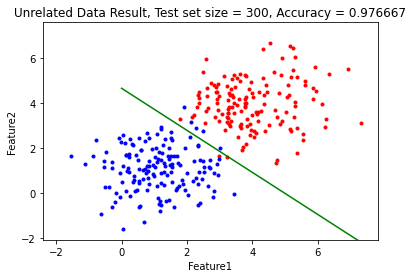
\includegraphics[width=0.6\textwidth]{Unrelated_Data_Result_Test.png}
    }
\end{figure}
可以看出模型的拟合效果较为准确,在训练集和测试集上表现均良好。
\subsection{实验数据不满足朴素贝叶斯假设}
与上一节类似的,我们只需要在生成数据时修改各个维度之间的协方差矩阵,使其维度之间不相互独立。同样生成1000个二维数据,设置超参数为$\lambda=0.002$,测试结果如下:
\begin{figure}[H]
    \centering
    \subfigure[不满足朴素贝叶斯假设的训练集测试结果]{
    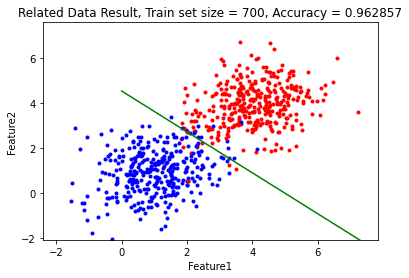
\includegraphics[width=0.6\textwidth]{Related_Date_Result_Train.png}
    }
    \subfigure[不满足朴素贝叶斯假设的测试集测试结果]{
    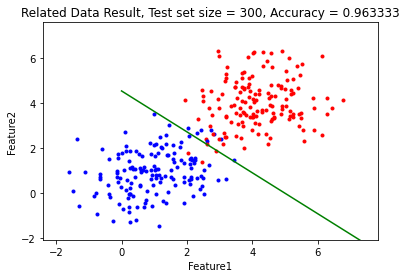
\includegraphics[width=0.6\textwidth]{Related_Data_Result_Test.png}
    }
\end{figure}
可以看出模型的拟合效果也较为良好,相较于满足朴素贝叶斯假设的数据,准确度有一定的下滑,但影响不大。
\subsection{使用UCI上的数据进行测试}
在此选择了UCI网站上的名为“banknote authentication Data Set”的数据集,其中包含了从真假钞图像中提取出的四个维度的特征数据,以及对真假钞的分类结果。数据集的摘要如下:
\begin{figure}[H]
    \centering
    \subfigure[数据集摘要]{
    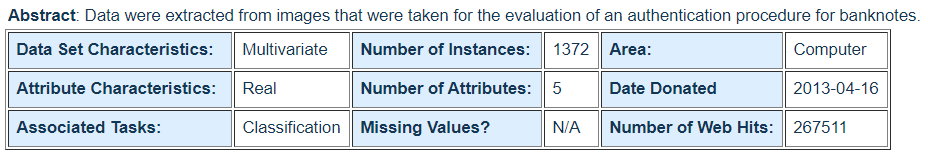
\includegraphics[width=0.8\textwidth]{UCI_Data_Abstarct.png} 
    }
\end{figure}
在读取数据之后,按照7:3的比例将其分割为训练集和测试集,最终模型的测试结果如下:
\begin{figure}[H]
    \centering
    \subfigure[UCI数据集分类结果]{
    
\includegraphics[width=0.8\textwidth]{UCI_Test_Result.png} 
    }
\end{figure}
由以上分类结果观察,该模型针对该数据集的分类效果较好。
\section{结论}
逻辑回归在一定程度上以较好的效果解决了基本的分类问题。其对于满足朴素贝叶斯假设的数据有着十分优秀的分类效果,但从实验结果上观察,该模型对于不满足朴素贝叶斯假设的数据也有着不俗的分类效果。\par
逻辑回归在现在仍然是一种高效的分类模型,我们利用该模型对于UCI上的数据集的分类效果也十分优秀。
\newpage
\end{document}